\subsection{Travel Planners for both individual and grouped travellers}

This section will analyse existing optimisation
techniques for TTDP solutions. These include
swarm-based, trajectory-based and evolutionary
algorithms. Gavalas et al.~\cite{Gavalas2014a}
classify TTDP variants into two; Systems that produce
a single route and systems that can handle multiple
days. 

Trip planner applications aim to offer tourists
information in a unified and centralised manner,
providing them with a plan for their trip. Two domains
develop current applications: methods for obtaining
POIs and tour recommendation algorithms that create
tourist trips, as shown in Figure \ref{RS}.

\begin{figure}[h]
\centering
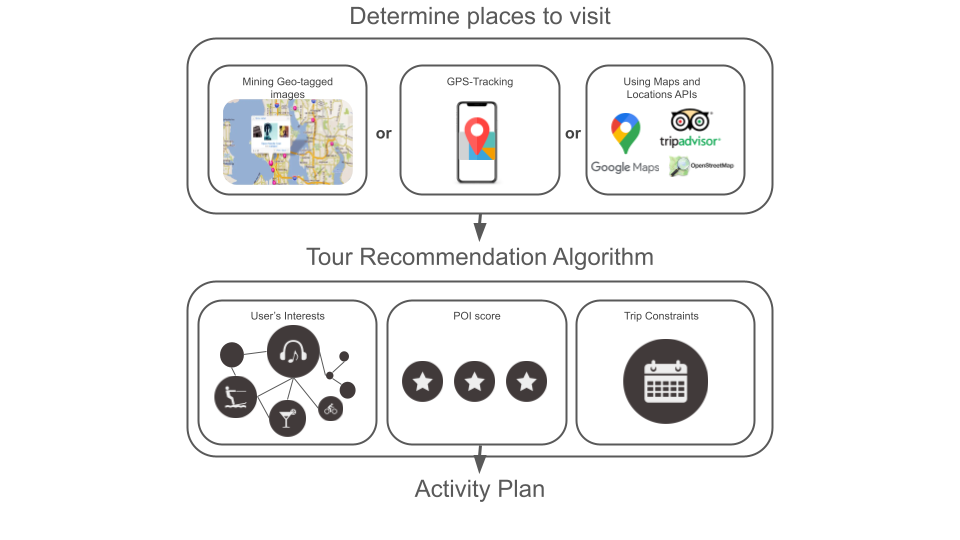
\includegraphics[width=1\textwidth]{RSProcess.png}
\caption{Trip Planner Applications Process.}
\label{RS}
\end{figure}

\subsubsection{Collecting the Points of Interests}

Before producing an itinerary, the tourist planners have to
formulate a dataset of POIs from some data source. There are
several ways to identify an appropriate data source representing
real-life tourist trajectories. 

One approach is made by gathering tourist places by mining them from
geotagged images of Location-Based Social Networks (LSBN) such as Flickr,
or Facebook ~\cite{DeChoudhury2010, Memon2015, Lucchese2012, Lim2018a,
HuiLim, HuiLima, Kurashima2013, Kurashima2010, Brilhante2013, Brilhante2015 }.

The ubiquitous presence of smartphones and GPS-enabled devices
could help gather the best POIs to visit based on other users'
historical paths~\cite{10.1145/1889681.1889683,
10.1145/1526709.1526816, Chen2011a}. However, privacy issues are the main caveat
towards this approach since it requires people to share their
location constantly and publically\cite{Lim2018}.

A prompt and accurate strategy towards gathering essential places
in the vicinity uses Mapping \& Location APIs such as Foursquare,
Google or TripAdvisor. Worndl et al.\cite{Worndl2017} use this approach and build a
dataset of prominent POIs by querying their API with the user's
desired location. In return, they receive a sequence of places and
information about each site, including its category, other user's
ratings, opening hours, coordinates and helpful additional
information to use as criteria for the itineraries.


\subsubsection{Single Route Problems}

The Orienteering Problem (OP), introduced by Tsiligirdes~\cite{Tsiligirides1984}, is the foundation of
single route planners in observance of the sport, orienteering. There are
various types of OPs that include different constraints, such as time windows
and time dependency, as shown in figure ~\ref{variants}. The OP can be represented as a
travelling salesman problem with profits. Gavalas et al. and Vansteenwegen et al.~\cite{Gavalas2014a, Vansteenwegen2011b}
mathematically formulate the OP as follows:




\setlength{\tabcolsep}{20pt}

Consider a set of POIs \[P = {p_1,p_2,\ldots,p_N}\]
where:
\\

\begin{tabular}{l l}


\textit{p}:  &  A POI having the latitude, longitude, category,\\
 & price, and corresponding set of opening hour constraints \\
 &\\
\end{tabular}
\\
The objective function of OP is:

\[ \text{MAX}  \sum_{i=2}^{N-1} \sum_{j=2}^{N} {s_i}{x_{ij}} \]
where:
\\
\begin{tabular}{l l}
% \textit{i,j}:  &  POI (\textit{i,j} = 2,3,...,\textit{N}) \\
\textit{$s_i$} & score of visiting node i \\
\textit{$x_{ij}$} & if a visit by POI i is followed by POI j (0 otherwise)\\

                  & \\
\end{tabular}


\textbf{Constraints} 

\begin{multicols}{2}
\begin{equation} 
    \label{constraintOne}
    \sum_{j=2}^{N} p_1j = \sum_{i=1}^{N-1} p_{iN}= 1
\end{equation}

\begin{equation} 
    \label{constraintTwo}
    \sum_{i=1}^{N-1} \sum_{j=2}^{N} t_{i}x_{ij}<= Tmax
\end{equation}


\end{multicols}

%\begin{multicols}{2}

\begin{equation} 
    \label{constraintThree}
    \sum_{i=1}^{N-1} x_{ir} = \sum_{j=2}^{N} x_{ij} \geq 1 \, \text{\small{r = 2, \ldots, N-1}}
\end{equation}

\begin{equation} 
    \label{constraintFour}
    2 \geq u_i \geq N 
\end{equation}
%\end{multicols}

\begin{equation} 
    \label{constraintFive}
    u_i - u_j + 1 \geq (N-1)(1-x_{ij})
\end{equation}

where:

\begin{tabular}{l l}
\textit{$t_{ij}$} & travel time from i to j \\
\textit{T} & maximum time \\
\textit{$u_i$} & position of POI i in route\\

               & \\

\end{tabular}


Constraint~\ref{constraintOne} ensures that the path starts at POI 1 and ends at POI N.
Constraint~\ref{constraintTwo} limits the total travel time.
Constraint~\ref{constraintThree} ensures that each POI is visited only once.
Constraint~\ref{constraintFour} and constraint~\ref{constraintFive} ensures that there are no subtours.
\\



% TODO: (Include Short Maths Formula, maybeone done by Kobeaga2018)


\begin{figure}[h]
\Tree [.{Orienteering Problem (Single Route)} .{Op with Time Windows}  {Time-Dependent OP} 
{Team OP (Multi-Route)} !{\qframesubtree} ]
\caption{Some Variants of the Orienteering Problem}
\label{variants}
\end{figure}

There are numerous Evolutionary Algorithms (EA) proposed to solve OP.\@
~\cite{Kobeaga2018,Wang2008}. EAs are algorithms based on natural evolution which
use a fitness score to get to the best solution of a problem, in this case, the
TTDP~\cite{Gunawan2016}.


%\centering
%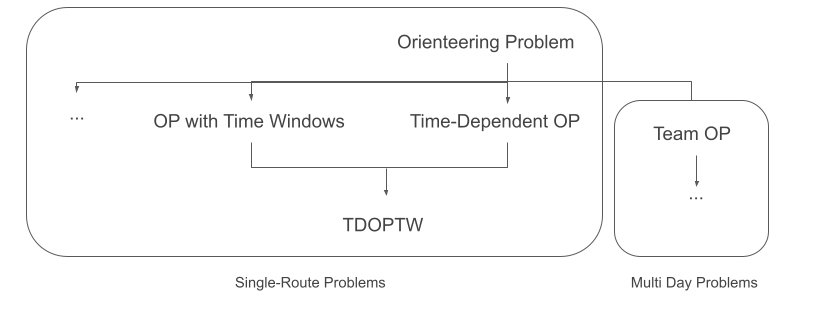
\includegraphics[width=0.5\textwidth]{TOP_graph.png}

Particle Swarm Optimisation-based (PSO) systems provide prevalent OP solutions
with fast computing time~\cite{Yu2019}. These are bio-inspired meta-heuristic approaches in
which, in the TTDP, a particle represents a travel path. The particles aim to
optimise themselves by communicating with each other and using their velocity
property to move to the most optimal solution~\cite{RezaeeJordehi2013}. Sevkli
et al.~\cite{Sevkli2010,Sevkli2010a} tested out two PSO variants:
Strengthened Particle Swarm Optimization (StPSO) and Discrete Strengthened
Particle Swarm Optimization (DStPSO). These two algorithms introduce pioneering
particles, which first perform a local search-based technique called Reduce
Variable Neighborhood Search (RVNS) between all the particles and then assign a
random velocity. These PSO algorithms obtains either the best or competitive
solutions compared with other algorithms such as Ant Colony and Genetic
Algorithms when tested on the Tsiligirides~\cite{Tsiligirides1984, Chen2011a} dataset of predefined nodes.

A novel approach in 2018  by Kobeaga et
al.~\cite{Kobeaga2018} was able to achieve
competitive solutions for medium-sized instances of
over 400 nodes and find new best-known solutions for
large datasets using the steady-state genetic
algorithm. The algorithm also implements a local
search, which aims to reduce travel time.

In 2019, Santini et al.~\cite{Santini2019} introduced a heuristic algorithm based on
adaptive extensive neighbourhood search. They evaluated their system by
comparing it with Kobeage et al.'s EA.\@ The results showed that both algorithms
find competing solutions in a reasonable amount of time. However, the EA finds
slightly more suitable solutions, while the extensive neighbourhood search has
a lower average gap.

In real-life scenarios, POIs have time constraints that allow them to be
visited only during specific hours, such as opening and closing hours or public
holiday constraints. Traditional OP is not able to cater for such problems. A
single route variant of the OP which solves these issues is the Orienteering
Problem with Time Windows (OPTW)~\cite{Gavalas2014a}. 

Kantor et al.~\cite{Kantor1992} provided the first attempt towards the
OPTW~\cite{Vansteenwegen2011}. They developed two algorithms;
Insertion and depth-first search. The former algorithm solves the path by
selecting a POI with the highest score over-insertion cost incrementally. On
the other hand, the depth-first search algorithm gathers parallel tree-based
solutions simultaneously and iteratively adds new POIs as long as they follow a
set of constraints. Their evaluation showed significant improvements of the
second algorithm over the insertion. 

When travelling between two POIs, the travel time may depend on certain
variable time constraints such as the traffic levels and waiting time~\cite{Herzog2020}.
The Time-Dependent Orienteering Problem (TDOP) introduced by Fomin et al.
~\cite{Fomin2002} is the single route variant of OP, which considers
these scenarios since traditional OPand OPTW does not~\cite{Gunawan2016}. In 2011, Abbaspour et
al.~\cite{Abbaspour2011}provide a solution for the
Time-Dependent Orienteering Problem with Time Windows, which combines the two
previously mentioned OP variants (TDOPTW).  They propose two adaptive genetic
algorithms and multi-modal shortest pathfinding evaluated in the city of
Tehran.


\subsubsection{Multiple Route Problems.}

The solutions available from what we discussed in the previous sections can only
generate a single efficient path for a tourist's holiday. The Team Orienteering
Problem (TOP)~\cite{Chao1996} is a variant of the OP, which allows for
solving the TTDP with multiple days~\cite{Sylejmani2017}. The system generates a full
itinerary for the tourist, with a maximum total score of all routes~\cite{Herzog2020}.

Several solutions use PSO-based algorithms to solve the TOP
~\cite{Muthuswamy2011,Wisittipanich2020,Yu2019}
Muthuswamy et al.~\cite{Muthuswamy2011} developed a discrete version of the PSO (DPSO)
which can generate n routes where $2 \geq n \geq 4$. The algorithm consists of two procedures;
Random initialisation of n-1 routes. The n\textsuperscript{th}
route is based on partial randomness and the current score divided by the current
distance of each particle after updating the velocity.  The
particles use RVNS and 2-opt techniques to communicate with each other as local
search techniques. The authors evaluated their work by comparing the algorithm
to seven TOP heuristics in which DPSO performed competitively across all
applied benchmark data sets~\cite{Gavalas2014a}.

A few years later, Dang et al.\ wrote another PSO inspired algorithm (PSOiA) for
the TOP.\@ They evaluated their work using an interval graph model, which showed
how to examine a more extensive search space faster~\cite{Gunawan2016}.

Besides swarm-based algorithms, an algorithm by Sylejmani et al.~\cite{Sylejmani2012}
used the trajectory-based tabu search to solve a Multi Constrained Team OPTW.\
Their system followed three steps in order to generate an activity plan: a new
activity is added as a node to the trip using \emph{Insert}, a node is
exchanged with a new activity using \emph{Replace} and two nodes swap with each
other using \emph{Swap}. 

%Several new applications use PSO-based solutions.
%In 2019, Yu et al.~\cite{Yu2019} developed a system for the Team OPTW variant based on
%selective DPSO.\@ In 2020, Wisittipanich\cite{Wisittipanich2020} presented an application of a
%metaheuristic called Global Local and Near-Neighbour Particle Swarm
%Optimization (GLNPSO). Wisittipanich evaluated their results using LINGO, an
%optimisation program and showed excellent results.


